% DS 7400 HW3 report. Build from docs/: tectonic -X compile hw3-report.tex  (or pdflatex; figures from ../results/hw3/)
\documentclass[10pt]{article}
\usepackage[letterpaper,margin=0.62in,top=0.55in,bottom=0.6in]{geometry}
\usepackage[T1]{fontenc}
\usepackage{lmodern}
\usepackage{microtype}
\usepackage{amsmath,amssymb}
\usepackage{booktabs}
\usepackage{graphicx}
\usepackage{xcolor}
\usepackage{tikz}
\usetikzlibrary{positioning,arrows.meta}
\usepackage[hidelinks]{hyperref}
\usepackage{enumitem}
\setlist{nosep,leftmargin=1.2em}
\setlength{\parskip}{2pt}
\setlength{\parindent}{0pt}
\usepackage{titlesec}
\titlespacing*{\section}{0pt}{5pt}{2pt}
\titleformat{\section}{\normalfont\bfseries\large}{\thesection}{0.5em}{}
\graphicspath{{../results/hw3/}}
\newcommand{\pp}{\,pp}

\begin{document}
\begin{center}
{\Large\bfseries Residual Gated Dual Pooling for a Mini-PointNet: a controlled test}\\[2pt]
Haeyun Choi \quad$\cdot$\quad DS 7400 Deep Learning, Homework 3 \quad$\cdot$\quad code: \texttt{feature/hw3-gated-pooling}
\end{center}
\vspace{-4pt}

\section{Background and observed limitation}
My HW2 classifier is a Mini-PointNet for ModelNet10 (10 furniture classes; 3{,}193 train / 798 validation / 908 test objects).
Each CAD mesh becomes \textbf{1{,}024 points sampled on its surface} (triangles chosen $\propto$ area); a point is only $(x,y,z)$, so a batch is a tensor of shape $(B,1024,3)$.
Points are centred and scaled into the unit sphere ($\hat p_i=(p_i-\mu)/\max_j\lVert p_j-\mu\rVert$), which removes translation \emph{and absolute size};
training adds an independent per-axis scale $\mathcal U(0.8,1.25)$, a shift and clipped jitter.
A shared per-point MLP ($3{\to}64{\to}128{\to}256$, Conv1d $k{=}1$, BatchNorm, ReLU) produces $h_i\in\mathbb R^{256}$, a \textbf{global max pool} $m_c=\max_i h_{i,c}$ makes the result order-invariant, and a head $256{\to}128{\to}10$ classifies (76{,}362 parameters; 92.77$\pm$0.60\% test accuracy over 3 seeds).
Its errors concentrate on look-alike pairs: in seed~0, \textbf{12 tables$\to$desk, 4 desks$\to$table, 11 dressers$\to$night stand and 11 night stands$\to$dresser} --- 38 of 58 errors.
These pairs differ mostly in proportion and extent. Max pooling keeps only the most extreme point per channel: it ignores \emph{how many} points show a feature (prevalence), how surface features are distributed, and $\partial m_c/\partial h_{i,c}=\mathbf 1[i=\arg\max]$ routes gradient to one point per channel.

\section{Hypothesis and proposed design (fixed before any HW3 run)}
\textbf{Hypothesis.} A learned, channel-wise blend of max and mean statistics improves the proportion-defined pairs; this is a testable guess, not a known cause.
Two course principles shape the design: \textbf{ResNet}~[1] --- keep a mapping that works as the identity path and learn a \emph{correction} around it; \textbf{SENet}~[2] --- squeeze global descriptors and learn a data-dependent \emph{channel-wise} sigmoid gate.
\textbf{Residual Gated Dual Pooling} (E2) keeps the max-pooled vector and adds a gated move toward the mean:
\[
m=\max_N h,\quad a=\operatorname{mean}_N h,\quad g=\sigma\!\big(W_2\,\mathrm{ReLU}(W_1[m;a]+b_1)+b_2\big),\quad z=m+g\odot(a-m)=(1-g)\odot m+g\odot a .
\]
$W_1{:}\,512{\to}16$, $W_2{:}\,16{\to}256$ (SENet's reduction ratio 16), +12{,}560 parameters. \textbf{Baseline-preserving initialisation}: $W_2{=}0$, $b_2{=}{-2}$, so training starts at $g=\sigma(-2)\approx0.119$ for every channel and object --- near max pooling, but outside sigmoid saturation. The head is unchanged.

\begin{center}
\resizebox{\linewidth}{!}{%
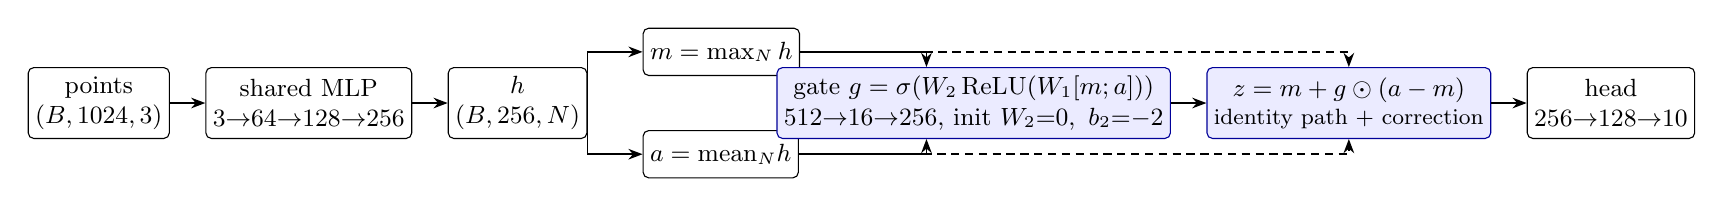
\begin{tikzpicture}[node distance=2.5mm and 4.5mm,
  box/.style={draw, rounded corners=2pt, align=center, font=\small, inner sep=2.5pt, minimum height=9mm},
  new/.style={box, fill=blue!8, draw=blue!60!black}, arr/.style={-{Stealth[length=1.8mm]}, semithick}]
  \node[box] (in) {points\\$(B,1024,3)$};
  \node[box, right=of in] (mlp) {shared MLP\\$3{\to}64{\to}128{\to}256$};
  \node[box, right=of mlp] (h) {$h$\\$(B,256,N)$};
  \node[box, right=7mm of h, yshift=6.5mm, minimum height=6mm] (m) {$m=\max_N h$};
  \node[box, right=7mm of h, yshift=-6.5mm, minimum height=6mm] (a) {$a=\mathrm{mean}_N h$};
  \node[new, right=24mm of h] (g) {gate $g=\sigma(W_2\,\mathrm{ReLU}(W_1[m;a]))$\\$512{\to}16{\to}256$, init $W_2{=}0,\ b_2{=}{-2}$};
  \node[new, right=of g] (z) {$z=m+g\odot(a-m)$\\[-1pt]{\footnotesize identity path + correction}};
  \node[box, right=of z] (head) {head\\$256{\to}128{\to}10$};
  \draw[arr] (in)--(mlp); \draw[arr] (mlp)--(h); \draw[arr] (h.east)++(0,0)|-(m); \draw[arr] (h.east)|-(a);
  \draw[arr] (m.east)-|([xshift=-6mm]g.north); \draw[arr] (a.east)-|([xshift=-6mm]g.south);
  \draw[arr] (g)--(z); \draw[arr] (z)--(head);
  \draw[arr, densely dashed] (m.east)-|(z.north); \draw[arr, densely dashed] (a.east)-|(z.south);
\end{tikzpicture}}
\end{center}
\vspace{-6pt}

\section{Controlled experiment}
Four conditions, seeds 0, 1, 2 (12 runs): \textbf{E0} the HW2 model rerun (max pool); \textbf{E1} fixed dual pool $z=0.5m+0.5a$ (no new parameters: does mean information help at all?); \textbf{E2} the proposed module (does \emph{learned} selection help?); \textbf{E3} max pool with width $h{=}69$, 88{,}537 parameters (is an E2 gain just its +16\% parameters?).
Held fixed: the cached 1{,}024 points per object and splits, augmentation, 60 epochs, batch 32, Adam (lr $10^{-3}$, weight decay $10^{-4}$), cosine schedule, dropout 0.3, checkpoint by validation accuracy, one test evaluation, package versions and CPU model (Xeon Gold 6248, 8 threads).
Within a seed every condition sees the same batches and augmentation, and E0/E1/E2 start from identical shared weights and dropout stream (the gate is built in a forked RNG state) --- only the pooling differs.
Decision rule written in advance: \emph{supported} only if E2 beats both E0 and E3 by $\ge$0.5\,pp (HW2 seed SD $\approx$0.6\,pp; one test object $=$ 0.11\,pp) and the critical-pair errors fall.

\section{Results (post-experiment observations)}
\textbf{Reproducibility:} E0 reproduces the stored HW2 runs \emph{exactly} (93.61 / 92.29 / 92.40\%, same selected epochs), so differences come from the change or from seed variability.

\begin{center}\small
\setlength{\tabcolsep}{4pt}
\begin{tabular}{lrrrrrrrr}
\toprule
 & & & \textbf{Test} & table & desk & dresser & night st. & Test acc.\\
Model & Params & Val acc. & \textbf{acc.} & $\to$desk & $\to$table & $\to$night st. & $\to$dresser & 256 points\\
\midrule
E0 max pool (HW2) & 76{,}362 & 97.70 & \textbf{92.77}\,$\pm$\,0.60 & 16.0 & 4.3 & 11.0 & 11.3 & 89.61\,$\pm$\,0.54\\
E1 fixed dual & 76{,}362 & 97.66 & \textbf{92.66}\,$\pm$\,0.26 & 11.3 & 4.7 & 11.7 & 12.3 & 89.83\,$\pm$\,0.05\\
E2 gated dual (ours) & 88{,}922 & 97.49 & \textbf{92.77}\,$\pm$\,0.32 & 16.7 & 4.3 & 8.3 & 15.3 & \textbf{90.75}\,$\pm$\,0.18\\
E3 max pool, $h{=}69$ & 88{,}537 & 97.41 & \textbf{91.81}\,$\pm$\,0.34 & 19.7 & 4.3 & 15.7 & 12.0 & 89.24\,$\pm$\,0.81\\
\bottomrule
\end{tabular}\\[1pt]
{\footnotesize Mean (\,$\pm$\,SD) over 3 seeds, \%; error columns are test objects (mean over seeds).}
\end{center}
\vspace{-4pt}
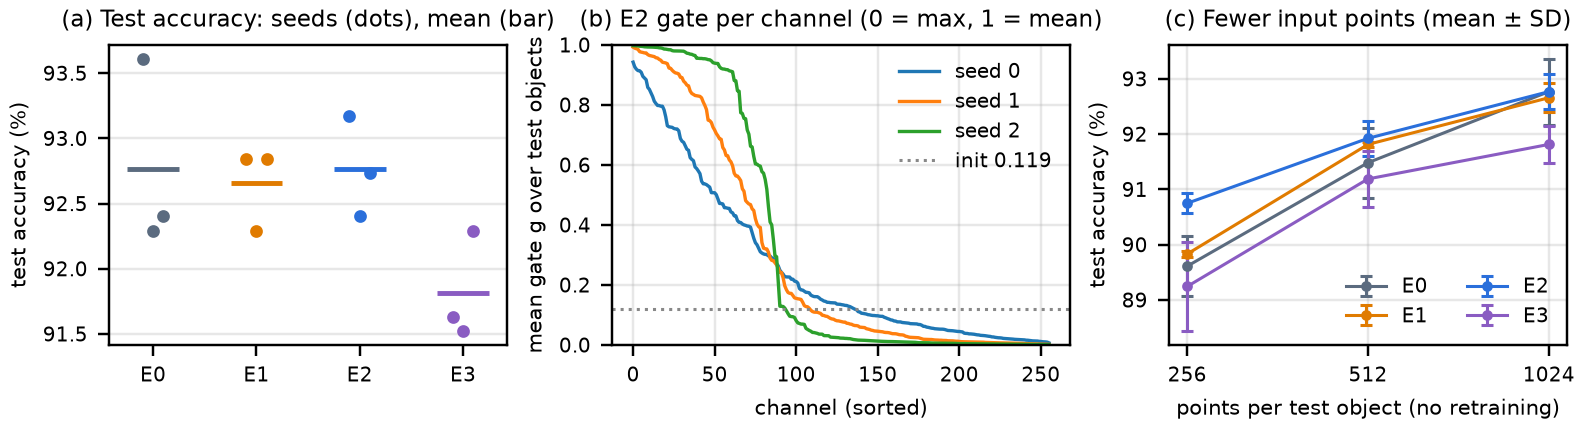
\includegraphics[width=\linewidth]{report_figure.png}
\vspace{-12pt}

\begin{itemize}
\item \textbf{Main hypothesis not supported.} Paired by seed, E2$-$E0 $=-0.44,+0.11,+0.33$\,pp (mean \textbf{+0.00}; exact McNemar $p=0.57,1.00,0.61$); E1$-$E0 $=-0.11$\,pp; E2$-$E1 $=+0.11$\,pp. The four critical errors did not fall (42.7$\to$44.7): E2 \emph{moved} the dresser/night-stand boundary ($-$2.7 / $+$4.0) instead of separating the pair. E3 is \emph{worse} than E0 ($-0.95$\,pp, 0/3 seeds), so capacity explains nothing and E2's +0.95\,pp over E3 is E3's deficit.
\item \textbf{The gate is used, but as a static channel split.} From 0.119 it became bimodal (b): 52--83 of 256 channels average $g>0.5$, while 43--62\% of gate values fell \emph{below} 0.1 toward pure max (weight decay, which pulls $g$ toward 0.5, cannot cause this split). Yet a channel's gate barely varies across objects (SD 0.006--0.017 vs.\ 0.27--0.42 across channels) and class means differ by $<$0.01: the SENet-style \emph{per-object} recalibration was not learned.
\item \textbf{A different, real benefit} (pre-registered secondary prediction): with 256 points per object E2 loses 2.0\,pp versus 3.2\,pp for E0, better in all 3 seeds (c) --- a max over fewer points shrinks, a mean does not. Gradient check: mean pooling reaches 100\% of points (max: 13\%), but the argmax points still carry 91--96\% of the per-point gradient norm.
\end{itemize}

\section{Failure analysis and next experiment}
\textbf{Why pooling could not fix the pairs.} A post-hoc probe (not pre-registered; no network) asks how well a single global cue separates each pair: the best threshold on one feature, chosen on the training pool, scored on the test split as balanced accuracy (50\% = chance).
\begin{center}\small
\begin{tabular}{llrl}
\toprule
Pair & Cue & Test bal.\ acc. & Removed or blurred by\\
\midrule
dresser vs.\ night stand & absolute height (raw mesh units) & \textbf{85.5\%} & normalisation (never in the input)\\
dresser vs.\ night stand & depth/width ratio & 81.4\% $\to$ \textbf{73.3\%} & per-axis scale augmentation\\
table vs.\ desk & any size or bounding-box ratio & 42--56\% & --- (not a global cue)\\
\bottomrule
\end{tabular}
\end{center}
\vspace{-3pt}
For dresser/night stand, absolute height alone is almost as good as the network's own within-pair accuracy ($\approx$87\%), and both strong cues are gone or blurred \emph{before} pooling, where no aggregator can recover them. For table/desk no global statistic helps: the difference is local structure (drawers, panels), which max pooling already targets, or label ambiguity. This matches what E2 did --- it learned to use mean statistics, yet the targeted errors did not move.

\textbf{Alternative explanations kept open.} Seed variability is large: paired runs that differ only in pooling still flip 15--39 test objects, so three seeds resolve about 1\,pp, not 0.1\,pp, and E3 shows that changing initialisation and width alone moves the score by $\sim$1\,pp (HW2's 93.6\% seed~0 was a favourable draw). The gate may also need an input that truly varies per object (e.g.\ the normalisation radius) to become data-dependent.

\textbf{Next controlled experiment.} \emph{E4}: E0 plus one scalar, $\log r$ (the normalisation radius, i.e.\ absolute size), concatenated to the pooled feature (+128 parameters), seeds 0--2, everything else fixed; primary outcome: dresser$\leftrightarrow$night-stand errors. Then \emph{E5}: isotropic scale augmentation (one factor for all axes) to test the augmentation explanation alone. Caveat: ModelNet sizes are per-model CAD units, and a size-aware model depends on the units of its inputs.

\textbf{Lesson.} A well-motivated module can be learned, can be used, and can still leave the target errors unchanged. The controls (E1, E3), the gate statistics and a cheap probe located the bottleneck in the input pipeline rather than in aggregation --- and revealed a side benefit (robustness to sparse inputs) that the clean accuracy hides.

{\footnotesize
\textbf{References.}
[1] K.~He, X.~Zhang, S.~Ren, J.~Sun, Deep Residual Learning for Image Recognition, CVPR 2016.
[2] J.~Hu, L.~Shen, G.~Sun, Squeeze-and-Excitation Networks, CVPR 2018.
[3] Z.~Wu et al., 3D ShapeNets (ModelNet), CVPR 2015.
[4] C.~R.~Qi et al., PointNet, CVPR 2017.
Code, all 12 runs, design record (committed before training) and full logs: repository \texttt{README.md}, \texttt{docs/hw3-design.md}, \texttt{docs/hw3-experiments.md}, \texttt{results/hw3/}.\par}

\end{document}
